%%%%%%%%%%%%%%%%%%%%%%%%%%%%%%%%%%%%%%%%%%%%%%%%%%%%%%%%%%
%%
%% MARK: Title
%%
%%%%%%%%%%%%%%%%%%%%%%%%%%%%%%%%%%%%%%%%%%%%%%%%%%%%%%%%%%

\chapter*{\S B21. The Use of the Moment Map in \hbox{Geodesic Calculus}}

%%%%%%%%%%%%%%%%%%%%%%%%%%%%%%%%%%%%%%%%%%%%%%%%%%%%%%%%%%
%%
%% MARK: Abstract
%%
%%%%%%%%%%%%%%%%%%%%%%%%%%%%%%%%%%%%%%%%%%%%%%%%%%%%%%%%%%

\begin{abstract}
  A fact or two about geodesics,
  proved thanks to the moment map.%
  \footnote{This note comes from a discussion with Jean-Paul Mohsen.}
\end{abstract}

%%%%%%%%%%%%%%%%%%%%%%%%%%%%%%%%%%%%%%%%%%%%%%%%%%%%%%%%%%
%%
%% MARK: On Geodesics
%%
%%%%%%%%%%%%%%%%%%%%%%%%%%%%%%%%%%%%%%%%%%%%%%%%%%%%%%%%%%

The moment map is a powerful tool in symplectic geometry.
This is another illustration.

\section{On geodesics}
\label{On-geodesics}

We consider the unparametrized geodesics of a Riemannian manifold $(M,g)$.
They are defined as the characteristics of the presymplectic $2$-form $d\lambda$ on the \emph{unit tangent bundle}:
$$%
  \UnitBundle{M} = \{(x,u) \in \TgtBundle M \mid x \in M,\ u \in T_x(M) \text{ and } u \cdot u = 1\},
  $$%
where $\TgtBundle M$ denotes the tangent bundle and $\lambda \in \DForms^1(\UnitBundle{M})$ is defined by its evaluation on a tangent vector $\delta(x,u) \in \Tgt_{(x,u)}(\UnitBundle{M})$:
$$%
  \lambda_{(x,u)}(\delta(x,u)) = u \cdot \delta x.
  $$%
We write $v \cdot w$ for $g_x(v,w)$,
and $\|v\|^2 = v \cdot v$,
where $v,w \in T_x(M)$.
The characteristics of $d\lambda$ satisfy the differential equations
$$%
  \delta(x,u) \in \ker(d\lambda_{(x,u)}) \quad \text{iff} \quad \delta x \propto u \quad \text{and} \quad \hat\delta u = 0,
  $$%
where $\hat\delta$ denotes covariant differentiation.
In a chart:
$$%
  \hat\delta u^\mu = \delta u^\mu + \Gamma^\mu_{\nu\rho} u^\nu \delta x^\rho,
  $$%
where $\Gamma^\mu_{\nu\rho}$ are the Christoffel symbols of the Levi-Civita connection.
The map $\delta(x,v) \mapsto (\delta x, \hat\delta v)$ is an isomorphism from $\Tgt_{(x,v)}(\TgtBundle M)$ to $T_x(M) \times T_x(M)$.
What we need to know now is this:

\begin{Article}{Geodesic trajectories.}{\itshape
  The integral curves of the distribution
  $$%
    (x,u) \mapsto \ker(d\lambda_{(x,u)})
    $$%
  project onto $M$ as the geodesic trajectories (or unparametrized geo\-de\-sics) of the Riemannian metric $g$.
  }
\end{Article}

Actually,
for every integral curve there always exists a parametrization $t \mapsto x(t)$,
defined on some interval,
such that $u(t) = dx(t)/dt$,
with $(x(t),u(t)) \in \UnitBundle{M}$,
and $[t \mapsto (x(t),u(t))]$ is a characteristic of $d\lambda$.
And that is how one usually understands the wording ``unparametrized geodesics''.

Now,
if a Lie group $H$ acts on $M$ preserving the metric $g$,
that is,
$h_M^*(g) = g$ for all $h \in H$,%
\footnote{When a group $H$ acts on a set $X$, we denote by $h_X \in \Perm(X)$ the action of $h \in H$ on $X$.}
then its natural action on $\TgtBundle M$ preserves $\UnitBundle{M}$:
$$%
  h_{\UnitBundle{M}}(x,u) = (h_M(x), h_{M*}(u) = \Der(h_M)(x)(u)),
  $$%
and also preserves $\lambda$ on $\UnitBundle{M}$:
$$%
  h_{\UnitBundle{M}}^*(\lambda) = \lambda.
  $$%
The moment map of this action is the pullback by the orbit map of the $1$-form $\lambda$ \cite{PIZ10},
that is,
$$%
  \mu(x,u) = [h \mapsto h_M(x,u)]^*(\lambda).
  $$%
Applied to a vector $Z$ in the Lie algebra $\cH$ of $H$,
this gives
$$%
  \mu(x,u) \cdot Z = u \cdot Z_M(x),
  $$%
where $Z_M(x)$ denotes the action of $Z$ on $M$,
that is,
the infinitesimal action of the $1$-parameter group generated by $Z$.

The \textbf{Noether theorem} states that the moment map is constant on the characteristics.
That means that if $[t \mapsto x(t)]$ is a geodesic with $u(t) = dx(t)/dt$ unitary,
then for all $t$ in the domain of the curve,
for all $Z \in \cH$,
$$%
  u(t) \cdot Z_M(x(t)) = u_0 \cdot Z_M(x_0),
  $$%
where $(x_0,u_0) = (x(t_0),u(t_0))$,
for an arbitrary $t_0$ in the domain of the curve.

%%%%%%%%%%%%%%%%%%%%%%%%%%%%%%%%%%%%%%%%%%%%%%%%%%%%%%%%%%
%%
%% MARK: Special Metrics on Principal Bundles
%%
%%%%%%%%%%%%%%%%%%%%%%%%%%%%%%%%%%%%%%%%%%%%%%%%%%%%%%%%%%

\def \UlOrthogonal {\underline{ortho}g\underline{onal}}

\section{Special metrics on principal bundles}

Consider now a principal bundle $\pi : M \to B$ with structure group $H$,
equipped with an $H$-invariant metric $g$.
Consider a connection on $M$ defined by orthogonal projectors:
for all $x \in M$ let $Q_x : T_x(M) \to T_x(H_M(x))$ be the vertical projector,
and $P_x = \Id_x - Q_x$ be the horizontal one.
In other words, the horizontal subspace is orthogonal to the fibers.
Assume also that the metric $g$ is ``calibrated vertically'',
meaning that there exists a left-invariant metric $\epsilon$ on $H$ such that
$$%
  \hat x^*(g) = \epsilon,
  \quad \text{i.e.} \quad g_x(Z_M(x),Z'_M(x)) = \epsilon(Z,Z'),
  $$%
where $\hat x$ is the orbit map:
$$%
  \hat x : H \to M
  \quad \text{with} \quad
  \hat x(h) = h_M(x).
  $$%
Now,
we have two interesting consequences of the conservation of the moment map along geodesics:

\begin{Article}{Proposition 1.}{}
  If a geodesic is horizontal at some point,
  it is horizontal at every point.
\end{Article}

\begin{proof}
  To be horizontal at a point means that the unit tangent vector $u_0$ is orthogonal to the fiber at $x_0$.
  Being orthogonal to a fiber at $t_0$ means:
  $u_0 \cdot Z_M(x_0) = 0$ for all $Z \in \cH$,
  since the vertical tangent space is spanned by the infinitesimal action of $H$.
  Then,
  since the moment map is constant along the geodesic,
  $u(t) \cdot Z_M(x(t)) = 0$ for all $t$.
  Hence the whole geodesic is horizontal.
\end{proof}

Actually this is a particular case of a more general property:

\begin{Article}{Proposition 1'.}{}
  Let $H$ be a group of isometries of $(M,g)$.
  If a geodesic is orthogonal to an orbit of $H$ at one point,
  it is orthogonal to every orbit it meets.
\end{Article}

In particular,
if the group has a fixed point,
every geodesic emanating from this point is orthogonal to every orbit it meets.
Consider for example the $2$-sphere,
and the rotations about an axis.
The poles are fixed and the geodesics passing through the poles are the meridians,
orthogonal to the parallels (the orbits of the rotations).

\begin{Article}{Proposition 2.}{}
  The fibers are totally geodesic.
\end{Article}

\begin{proof}
  Recall that being totally geodesic means that a geodesic which is tangent to a fiber at some point is tangent to that fiber at every point.
  
  Let $\{Z_i\}_{i=1}^k$ be an orthonormal basis of $\cH$,
  with respect to the metric $\epsilon$.
  Then,
  according to the hypothesis $\hat x^*(g) = \epsilon$,
  the vectors $Z_{i,M}(x)$ form an orthonormal basis of $T_x(H_M(x))$,
  for all $x \in M$.
  Let $t \mapsto x(t)$ be a geodesic with unitary velocity $u(t)$,
  and write $u(t) = u_Q(t) + u_P(t)$,
  where $u_Q$ is the vertical part and $u_P$ the horizontal part.
  Then,
  $\|u_Q(t)\|^2 = \sum_{i=1}^k u_i(t)^2$,
  with
  $u_i(t) = u(t) \cdot Z_{i,M}(x(t))$.
  Thus,
  since the $u_i(t)$ are constant along the geodesic,
  $\|u_Q(t)\|^2$ is also constant along the geodesic.
  Hence,
  if $u_P(x_0) = 0$,
  then $\|u_Q(t)\|^2 = \|u_Q(0)\|^2 = 1$ for all $t$,
  and consequently $\|u_P(t)\|^2 = 0$.
  Therefore,
  if the geodesic is tangent to the fiber at some point, it is tangent everywhere.
\end{proof}

\begin{Article}{Remark.}{}
  On $\RR^2$ the standard metric is $\SO(2,\RR)$-invariant.
  And if we remove the origin,
  the action of $\SO(2,\RR)$ is principal.
  The geodesics are the lines and the orbits are the circles centered at the origin.
  A line which is tangent to a circle somewhere is not tangent to any other circle.
  Thus, the orbits are not geodesics.
  So? Did we miss something?
  It happens that the metric is not calibrated with respect to the action of $\SO(2,\RR)$.
  Precisely, $\hat x^*(g) = \|x\|^2 \epsilon$.
  Hence,
  we see that for Proposition 2,
  the hypothesis that the metric be calibrated is crucial.
\end{Article}

\vfill
%\centerline{\includegraphics[width=.36\textwidth]{Esher.jpg}}
\centerline{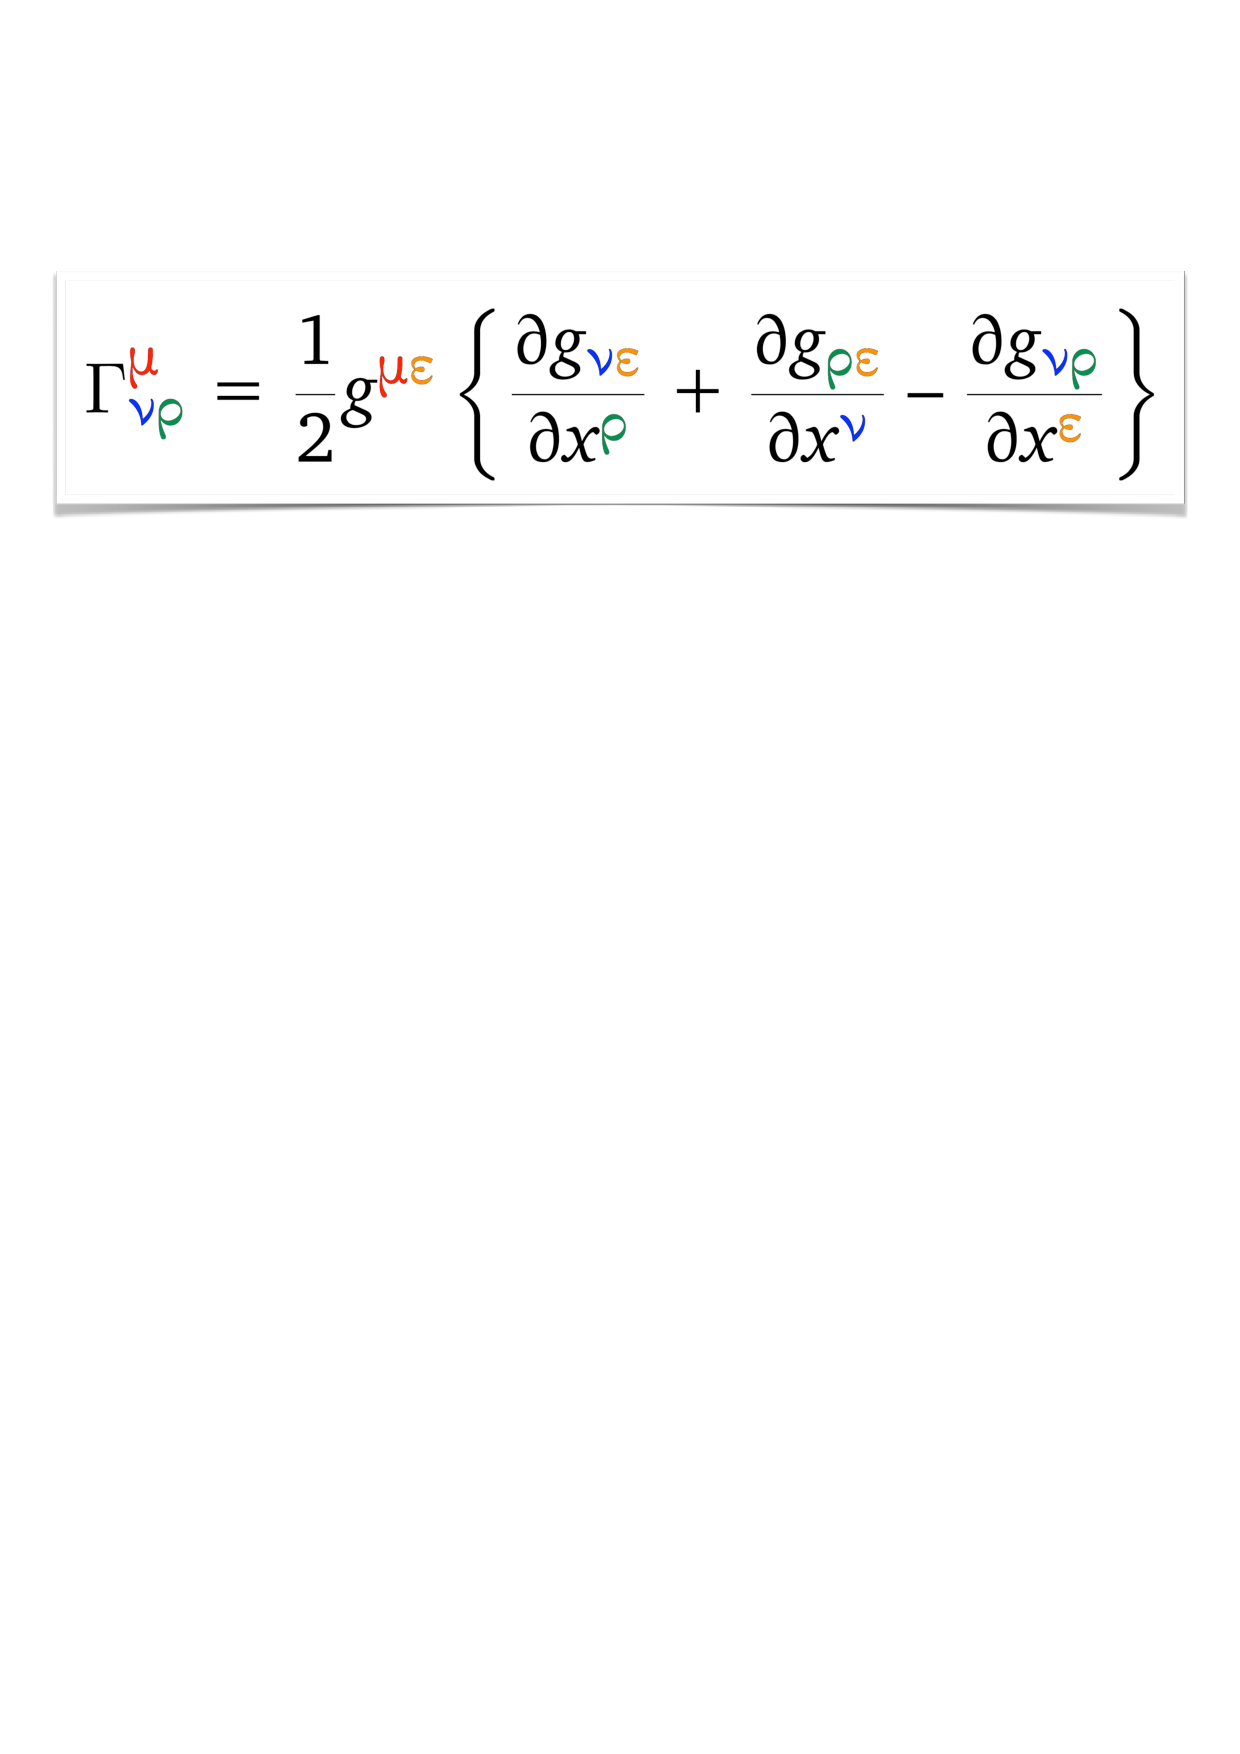
\includegraphics[width=\textwidth]{Figures/Christoffel.pdf}}
